\chapter{Desarrollo}
    \section{Proceso de medición}
         \subsection{equipos de medición}
            El equipo con el cual se tomo mediciones corresponde al usado por el departamento de \textit{System \& Optics} a cargo del ingeniero Sebastien Poupar, quien facilito el equipo para llevar a cabo las mediciones. Este esta compuesto de:           
            
            \vspace{0.5cm}
            \textbf{Amplificador Br\"uel \& Kj\ae r}
            \begin{itemize}
                \item Modelo: NEXUS tipo 2692-OS4.
                \item máximo de 4 canales.
                \item factor de amplificacion usado: $1 \left[\frac{V}{ms^{-2}}\right]$.
            \end{itemize}
            \begin{figure}[H]
                \centering
                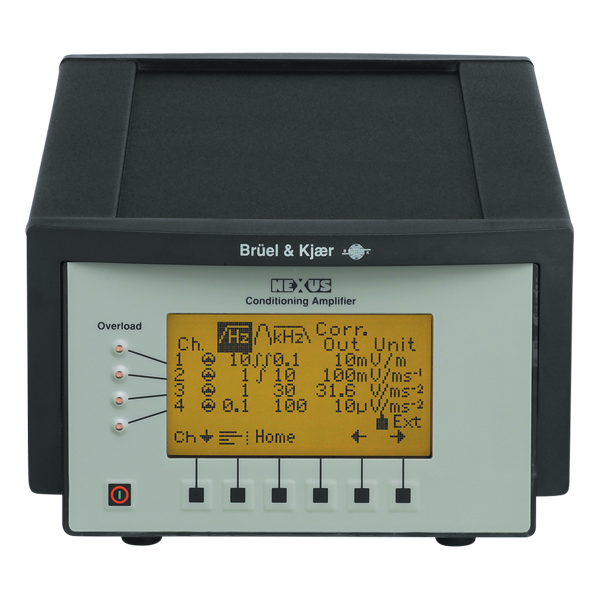
\includegraphics[width=0.3\linewidth]{Nexus}
                \caption{Amplificador Nexus 2692-OS4}
                \label{fig:NEXUS}
            \end{figure}
            \vspace{0.5cm}
            \textbf{Acelerometro Br\"uel \& Kj\ae r}
            \begin{itemize}
                \item Modelo 4370.
                \begin{itemize}
                    \item Alta sensibilidad.
                    \item Apto para vibraciones a baja frecuencia.
                    \item Frecuencia inferior: Determinada por la amplificación usada
                    \item Frecuencia superior: $4.8 [kHz]$
                    \item Frecuencia resonante: $17.7 [kHz]$
                \end{itemize}
                \item Cable modelo AO 0038
                \item cuatro ocupados
            \end{itemize}
            \begin{figure}[H]
                \centering
                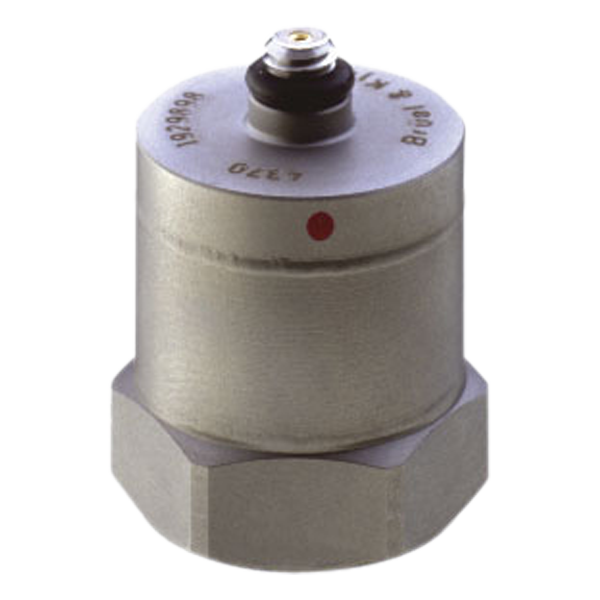
\includegraphics[width=0.15\linewidth]{4370}
                \caption{Acelerometo TYPE 4370}
                \label{fig:4370}
            \end{figure}
            \vspace{1cm}
            \textbf{Osciloscopio TiePie}
            \begin{itemize}
                \item Modelo HandyScope HS4.
                \item Resolución 4 bits.
                \item Sampling rate máximo de $5\left[\frac{Ms}{s}\right]$
                \item conexión a computador mediante USB
                \item Programa dedicado llamado \textit{MultiChannel Measurement TiePie}
            \end{itemize}
			\begin{figure}[H]
				\centering
				\begin{subfigure}[b]{0.45\textwidth}
					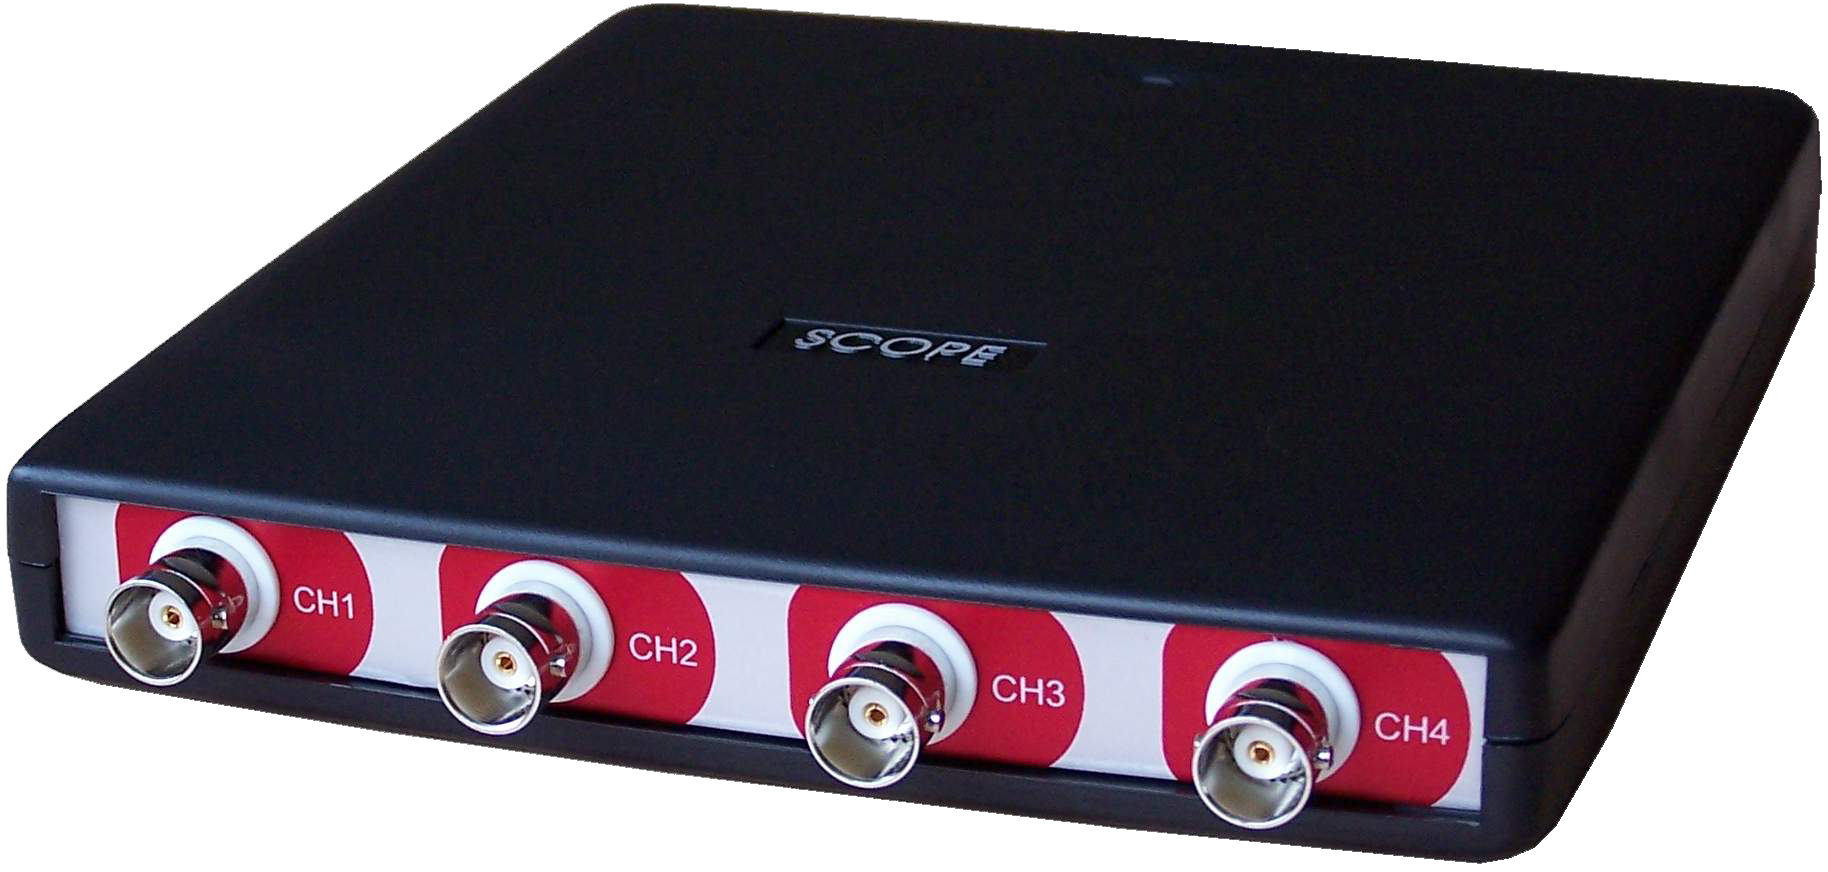
\includegraphics[width=0.7\textwidth]{handyscope}
					\caption{Osciloscopio HS4}
					\label{fig:handyscopehs4}
				\end{subfigure}			    
			    \begin{subfigure}[b]{0.45\textwidth}
			    	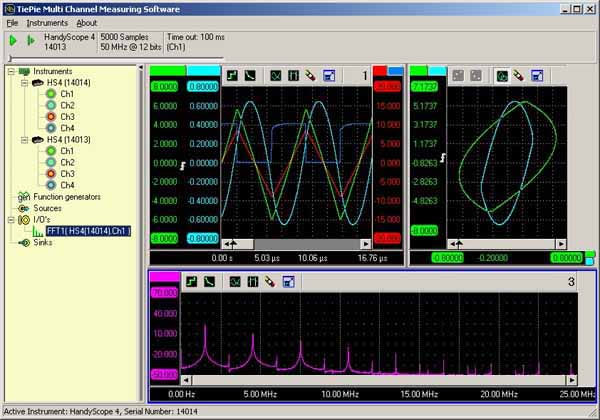
\includegraphics[width=0.7\textwidth]{tiepiesoftware}
			    	\caption{Programa Dedicado al osciloscopio}
			    	\label{fig:tiepiesoftware}
			    \end{subfigure}
		    \caption{Osciloscopio y programa}
		    \label{fig:osciloscopioyprograma}
		    \end{figure}
	    \subsection{Modo de medición}
	        \subsubsection{Configuración de la medición}
	            Uno de los problemas de medir RTM es bajo la situación a la que operan que corresponde exclusivamente a las noches de observación. Implicando que en el día estos permanecen sin operar. Esto lleva a que en todas las mediciones se deba solicitar un telescopio y habilitar el sistema de RTM para su giro, por lo que es importante tener un plan de medición con la finalidad de tener mediciones comparables entre RTM y tener la mayor cantidad de información posible al hacer girar el enclosure.
	            
	            \vspace{0.5cm}
	            \textit{\textbf{Velocidad de rotación del enclosure:}}
	            \vspace{0.5cm}
	            
	            El rango de velocidades en el que puede operar el enclosure es de $[0-2][\frac{^{\circ}}{seg}]$, dentro de este rango se toma $1 [\frac{^{\circ}}{seg}]$ por medidas de seguridad ya que es una masa de $280.000[kg]$ con la que se trabaja. Este valor de medición significa que un giro del enclosure demora seis minutos.
	            
	            \vspace{0.5cm}
	            \textit{\textbf{Frecuencia de muestreo:}}
	            \vspace{0.5cm}
	            
	            La frecuencia de muestreo debe satisfacer dos condiciones:
	            \begin{enumerate}
	                \item La respuesta en  frecuencia (valor medicion/ valor real) debe ser bajo
	                \item Las muestras totales de un giro de enclosure no deben llenar el buffer interno del osciloscopio
	            \end{enumerate}
	            Tomando como prioridad el buffer del osciloscopio el cual es de $2[Ms]$ se calcula una tasa de muestreo de $5.5[kHz]$
	            
	            
	        \subsubsection{Donde medir}
	            \begin{figure}[H]
	                \centering
	                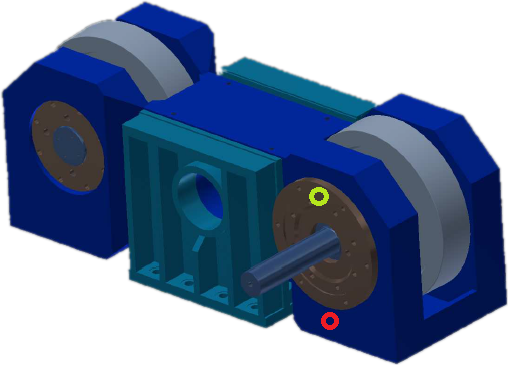
\includegraphics[width=0.5\linewidth]{rtm07mediciones}
	                \caption{Lugares de medición sobre RTM, colores corresponden a color del gráfico de frecuencias}
	                \label{fig:rtm07dondemidio}
	            \end{figure}
	            Uno de los puntos importantes al momento de realizar una buena medición es el de seleccionar lugares cercanos y rígidos donde montar los sensores, consultando a los planos \ref{fig:planodrivewheel} de diseño de RTM se identifica la tapa como punto de contacto directo para realizar las mediciones (Cuadrado rojo indica lugar del balancín). Haciendo una primera prueba, tomando mediciones en la tapa y en el cuerpo de acero del RTM07 de UT4 \footnote{Se hace medicion sobre este RTM aprovechando el desmontaje de su motor/reductor} se obtienen los espectros de frecuencia de la figura \ref{fig:plottapas}. Se observa que hay una disminución en las frecuencias medias y altas por lo que las tapas no son un buen punto sobre el cual medir. Otro factor que hace descartar a las tapas como punto de medición es que en terreno se comprueba que existen tapas con problemas de diseño como también pernos sueltos.
	            \begin{figure}[H]
	                \centering
	                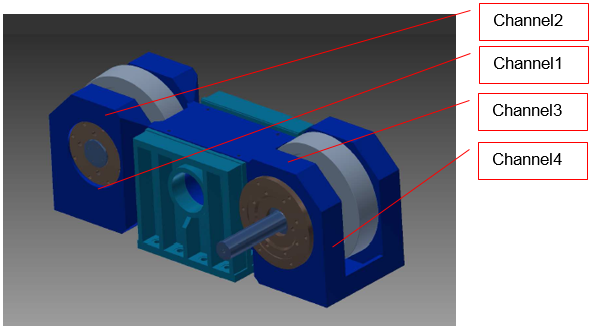
\includegraphics[width=0.6\linewidth]{lugarmedicionfinal}
	                \caption{Lugar final donde se realizan mediciones en todos los RTM}
	                \label{fig:lugaresdemedicionfinal}
	            \end{figure}
	            
	            Otro punto que juega en contra en las mediciones de RTM es el lugar en el cual están montados, imposibilitando la medición sobre la parte posterior debido a que están colocados en la periferia del enclosure teniendo un espacio confinado donde está el anillo que energiza los sistemas de enclosure. Esto hace que sea muy dificultoso y peligroso trabajar ahí. Por las razones mencionadas se decide por medir sobre el balancín (estructura de acero) como se muestra en la figura \ref{fig:lugaresdemedicionfinal}
	            \begin{figure}
	                \centering
	                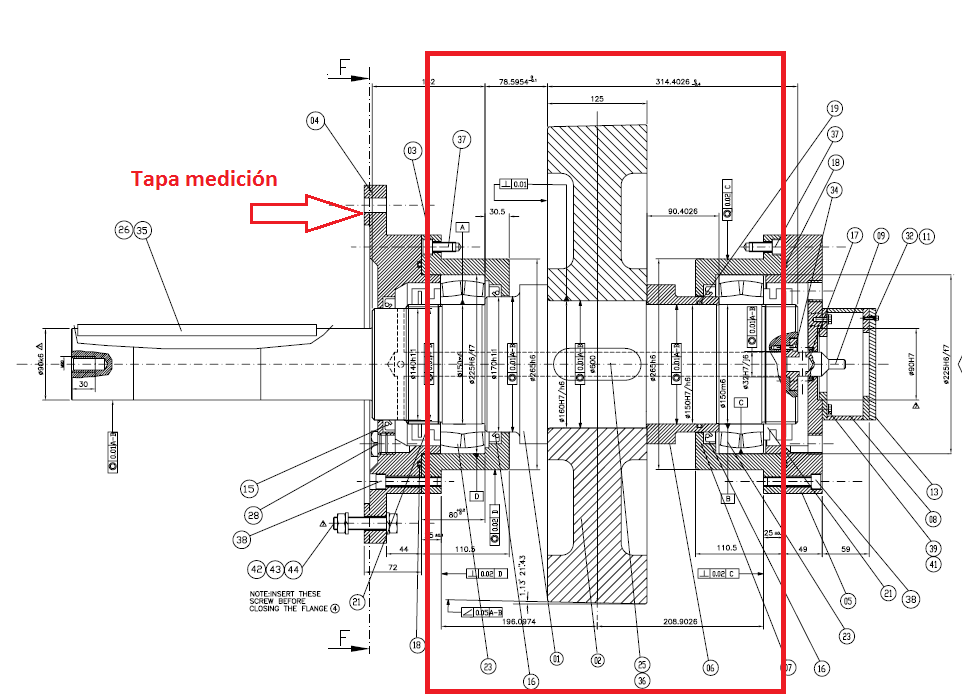
\includegraphics[width=0.8\linewidth]{drivewheel}
	                \caption{Plano Conjunto Drive Wheel}
	                \label{fig:planodrivewheel}
	            \end{figure}
	            \begin{figure}[H]
				    \centering
				    \begin{subfigure}[b]{\textwidth}        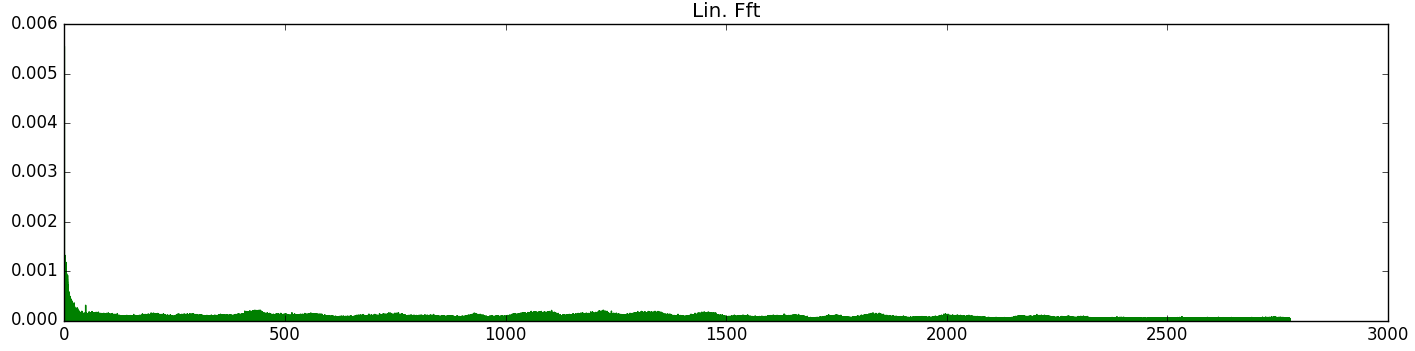
\includegraphics[width=\textwidth]{plottapa1}
    					\caption{Medición sobre tapa}
    					\label{fig:plottapa1}
    				\end{subfigure}			    
    			    \begin{subfigure}[b]{\textwidth}
    			    	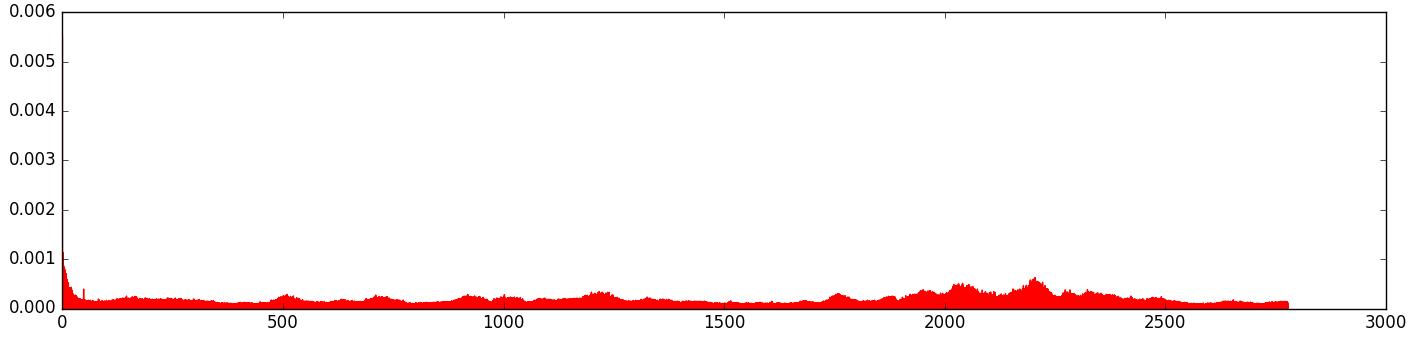
\includegraphics[width=\textwidth]{plottapa2}
    			    	\caption{Medicion sobre balancín}
    			    	\label{fig:plottapa2}
    			    \end{subfigure}
    		        \caption{Espectros obtenidos en prueba de tapa en UT4@RTM07}
    		        \label{fig:plottapas}
		        \end{figure}
		        
		        Resumiendo:
		        \begin{table}[H]
		            \centering
		            \caption{Tabla resumen para mediciones}
		            \begin{tabular}{|c|c|}
		                \hline
		                 Item & Detalle  \\ \hline \hline
		                 Frecuencia de Sampleo & 5555[Hz] \\ \hline
		                 Velocidad de Giro & $1\left[\frac{^\circ}{seg}\right]$ \\ \hline
		                 Vueltas de enclosure & 1 \\ \hline
		                 Velocidad de Ruedas & $8.2 [Rpm]$ (empírico) \\ \hline
		            \end{tabular}
		            \label{tab:resumenmedicion}
		        \end{table}
    \section{Análisis de impacto del riel sobre las mediciones}
        Uno de los factores que afectan la medición es la configuración y estado del riel. Al igual que el efecto explicado con anterioridad sobre el efecto campana producido en rodamientos es el que se espera en una configuración rueda-riel con imperfecciones. Debido a la alta carga con la que se trabaja, cualquier picadura o imperfección en la pista o rueda, generará una señal de impacto en la señal. Es por esto que se toma una medición prueba para ver como responde el sistema al tener un giro del domo.
        \begin{figure}[H]
            \centering
            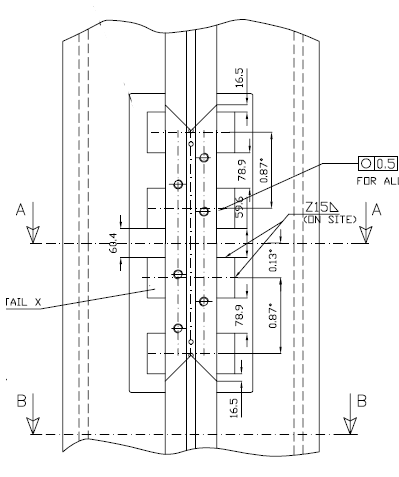
\includegraphics[width=0.6\linewidth]{detalleriel}
            \caption{Detalle de una unión de riel}
            \label{fig:unionesderiel}
        \end{figure}
        
        La estructura del domo, como se ve en la figura \ref{fig:topRTM}, el domo posee un riel curvado, de un diametro de $28.12 [m]$ de diámetro, el cual posee nueve uniones de segmentos (Figura \ref{fig:unionesderiel}), como se observa, cada sección se une con una sección menor la que va apernada a una viga, generandose dos secciones (entre viga) con sección de forma de V, lo que se pretende con la medición es ver si se generan impactos al pasar las uniones con el riel y ver como se comportan estas bajo un apriete de sus pernos de fijación. 
        
        
        Esta prueba se realizó en RTM08 de UT2 debido a la posibilidad de monitorear mejor sus condiciones ya que al momento de la medición se encontraba con el motor/reductor desacoplado. Se toman los datos para una vuelta y se guardan los datos en formato .Csv para su análisis en Python.
        \begin{figure}[H]
            \centering
            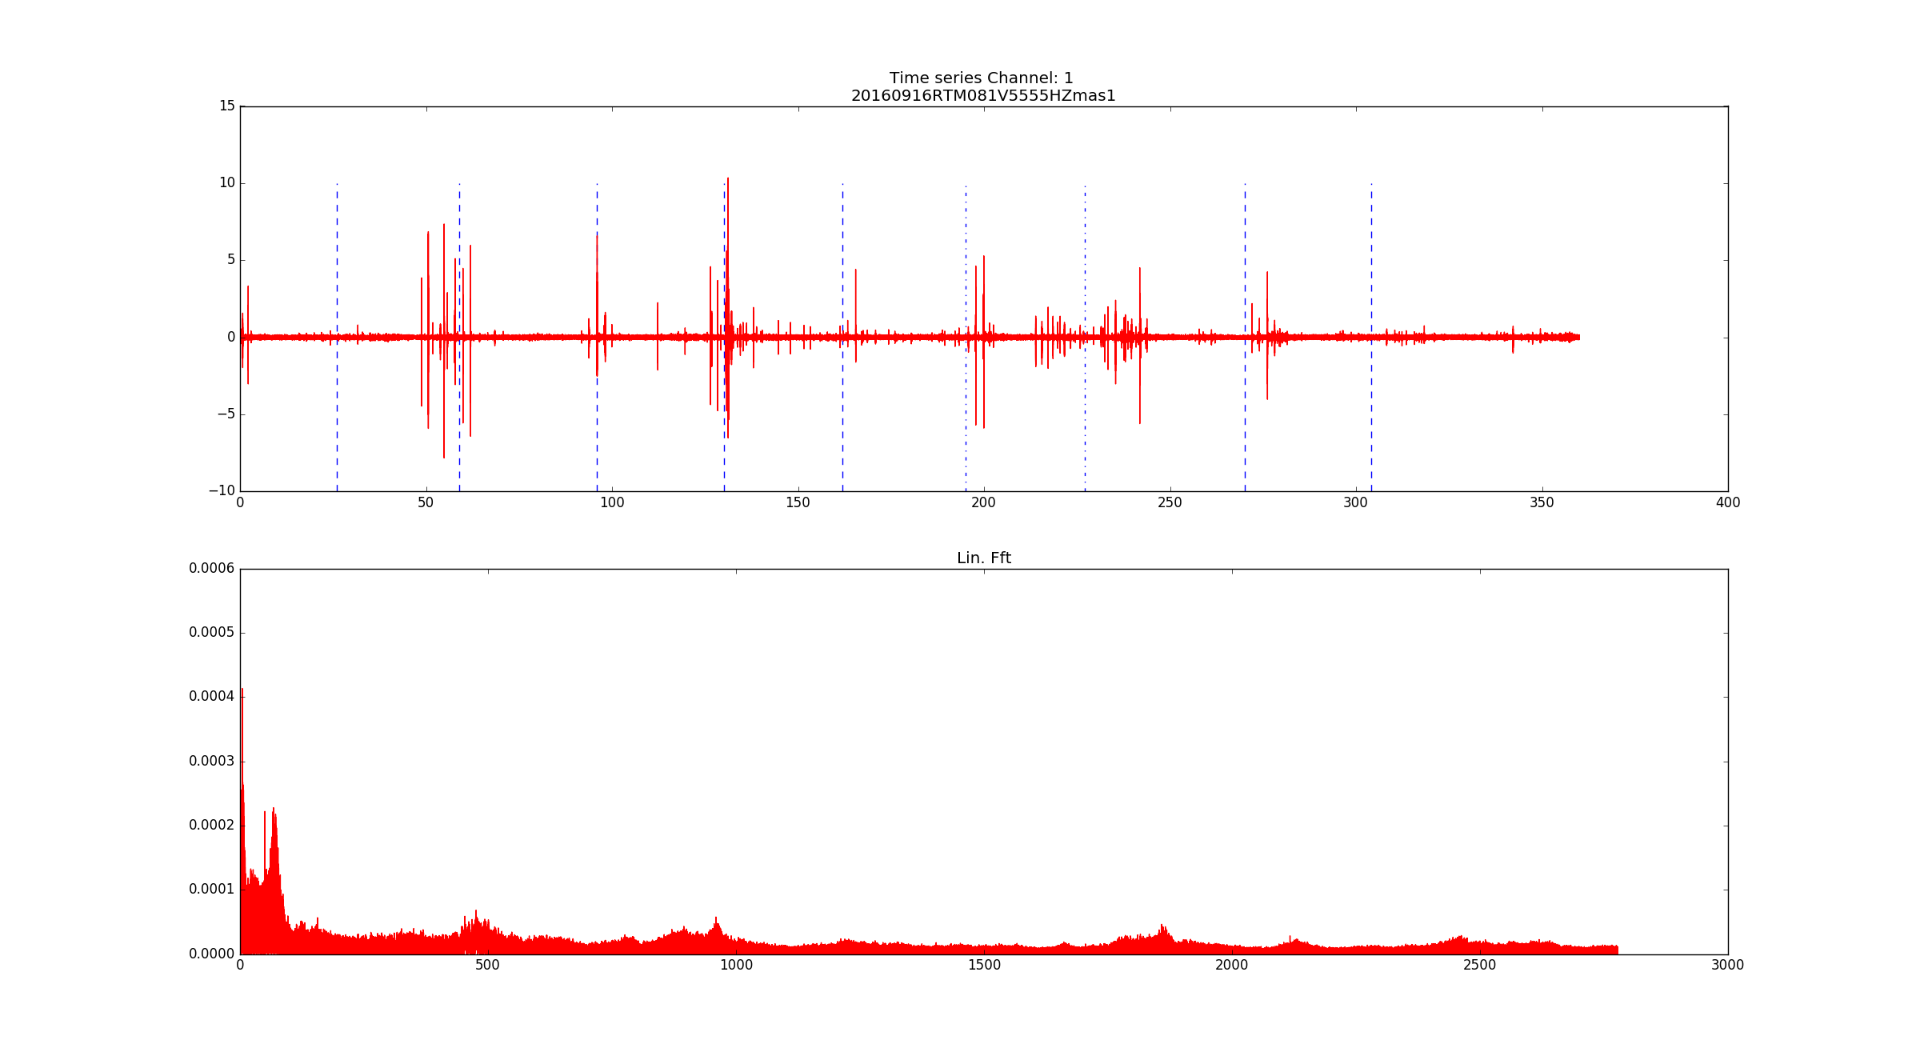
\includegraphics[width=\linewidth]{impactorielantes}
            \caption{Serie de Tiempo y FFT, análisis de impactos del riel}
            \label{fig:impactorielantes}
        \end{figure}
        
        En la figura \ref{fig:impactorielantes} se grafican los resultados, las lineas segmentadas indican el tiempo en el cual las ruedas chocan con una de las ruedas del RTM, se ve una dependencia clara con algunas zonas de altos impactos por lo que se procede a solicitar un apriete de pernos de unión para ver como se comporta el sistema al aplicar el apriete especificado por recomendado por el diseñador. Los resultados se muestran en la figura \ref{fig:impactorieldespues}
        \begin{figure}[H]
            \centering
            \includegraphics[width=\linewidth]{impactorieldespues}
            \caption{Serie de Tiempo y FFT para RTM despues de apriete de pernos de sujeción}
            \label{fig:impactorieldespues}
        \end{figure}
        
    \section{Resultado de mediciones}        
        \subsection{Análisis usando promedios en frecuencia}
            Para el análisis de resultados mediante esta técnica, se usa programa Python junto a las bibliotecas Numpy para trabajar con series de datos, Pandas para estructurar los datos de los 4 canales de medición (tipo DataFrame) y scipy para realizar transformada de fourier y algoritmo Welch para el calculo de la PSD. La manera en la que se entregan los datos es genérico mediante Jupyter. Herramienta con programación en Python con la posibilidad de agregar texto a modo de informe (Se agrega en anexos)
            \subsubsection{Algoritmo}
                Las finalidades del algoritmo son:
                \begin{enumerate}
                    \item Eliminar los impactos que se generan en una vuelta del enclosure para el calculo de la PSD
                    \item Hacer promedios en espectro de frecuencia para reducir el ruido y señales aleatorias, obteniendo peaks mas definidos en la PSD
                \end{enumerate}
                
                Esto se logra al seguir los siguientes pasos:
                
                \begin{itemize}
                    \item Capturan datos, salvan en un .csv (comma separated values)
                    \item Abre archivo a analizar y se estructuran datos en pandas.
                    \item Se hace un recorrido dato por dato, verificando que el dato no supere un valor definido (mayor a $1.5 [\frac{m}{s^2}]$).
                    \item Si el valor es mayor, se termina el largo de un arreglo y luego se suma un $\Delta t$ de tiempo del largo del impacto (calculado por medición).
                    \item Se continua buscando arreglos hasta que se terminan los datos.
                    \item De los N arreglos, se seleccionan aquellos que sean mayor a 40000 muestras para tener una buena resolución en frecuencias. En caso de poder dividirse en 2 o mas arreglos, se separan dejando solo arreglos de cuarenta mil datos (a mayor tiempo de adquisición, mejor la resolución en frecuencia).                    
                    \item Aplica PSD en todos los arreglos y se promedian
                    \item Se gráfica el resultado final
                \end{itemize}
		        